% ----------------------------------------------------------
% ELEMENTOS PÓS-TEXTUAIS
% ----------------------------------------------------------
% Retire o comentário somente se o padrão exigir que daqui para a
% frente não haja número de páginas.
%\postextual
% ----------------------------------------------------------

% ------
\bibliography{8-referencias/arquitetura,8-referencias/ferramentas-sws,8-referencias/tecnologias,8-referencias/notacaovisual,8-referencias/servicosweb,8-referencias/sistemascolaborativos,8-referencias/sws,8-referencias/estudo-de-caso,8-referencias/semantica-openapi,8-referencias/semantica-wadl}
% ------

% ----------------------------------------------------------
% Glossário
% ----------------------------------------------------------
%
% Consulte o manual da classe abntex2 para orientações sobre o glossário.
%
%\glossary

% ----------------------------------------------------------
% Apêndices
% ----------------------------------------------------------

% ---
% Inicia os apêndices e anexos
% ---
%\begin{apendicesenv}

% Imprime uma página indicando o início dos apêndices
\partapendices

\chapter{Estrutura Analítica de Projetos}\label{apendice-eap}

A estrutura analítica de projetos (EAP) da ferramenta Grasews é apresentada em quatro (4) partes. A \figurename~\ref{fig:grasews-eap-usuario} ilustra os sub-pacotes de trabalho e atividades a fim de entregar o pacote de trabalho denominado \texttt{Usuário}. A \figurename~\ref{fig:grasews-eap-wsdl} ilustra os sub-pacotes de trabalho e atividades a fim de entregar o pacote de trabalho denominado \texttt{WSDL}. A \figurename~\ref{fig:grasews-eap-owl} ilustra os sub-pacotes de trabalho e atividades a fim de entregar o pacote de trabalho denominado \texttt{OWL}. Finalmente, a \figurename~\ref{fig:grasews-eap-colaboracao} ilustra os sub-pacotes de trabalho e atividades a fim de entregar o pacote de trabalho denominado \texttt{Colaboração}.

%\begin{landscape}
    \begin{figure}[h]
        %\resizebox{\textwidth}{!}{
            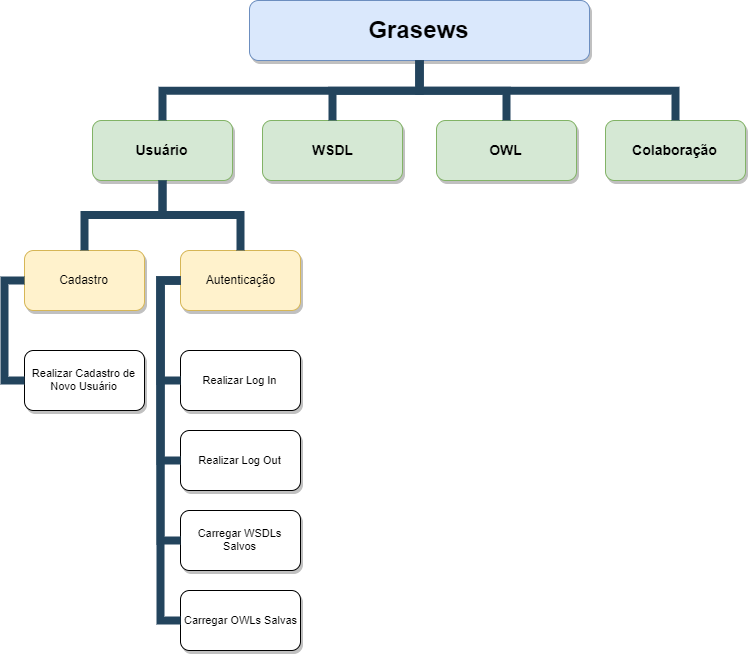
\includegraphics[scale=0.5]{9-pos-textuais/apendices/imagens/grasews-eap-usuario.png}
        %}
        \centering
        \caption[Estrutura Analítica de Projetos de Grasews - Parte 1]{\textbf{Estrutura Analítica de Projetos de Grasews - Parte 1.}}
        \label{fig:grasews-eap-usuario}
    \end{figure}
%\end{landscape}

%\begin{landscape}
    \begin{figure}[h]
        %\resizebox{\textwidth}{!}{
            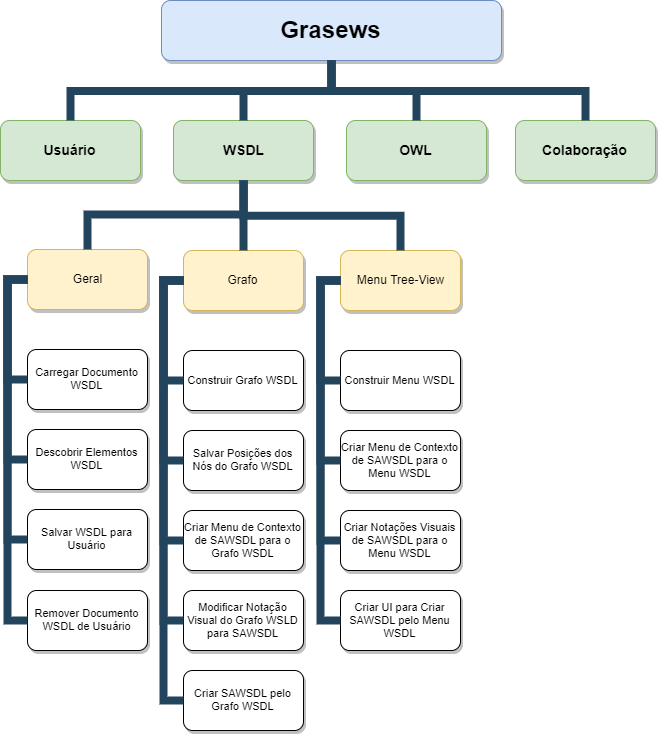
\includegraphics[scale=0.45]{9-pos-textuais/apendices/imagens/grasews-eap-wsdl.png}
        %}
        \centering
        \caption[Estrutura Analítica de Projetos de Grasews - Parte 2]{\textbf{Estrutura Analítica de Projetos de Grasews - Parte 2.}}
        \label{fig:grasews-eap-wsdl}
    \end{figure}
%\end{landscape}

%\begin{landscape}
    \begin{figure}[h]
        %\resizebox{\textwidth}{!}{
            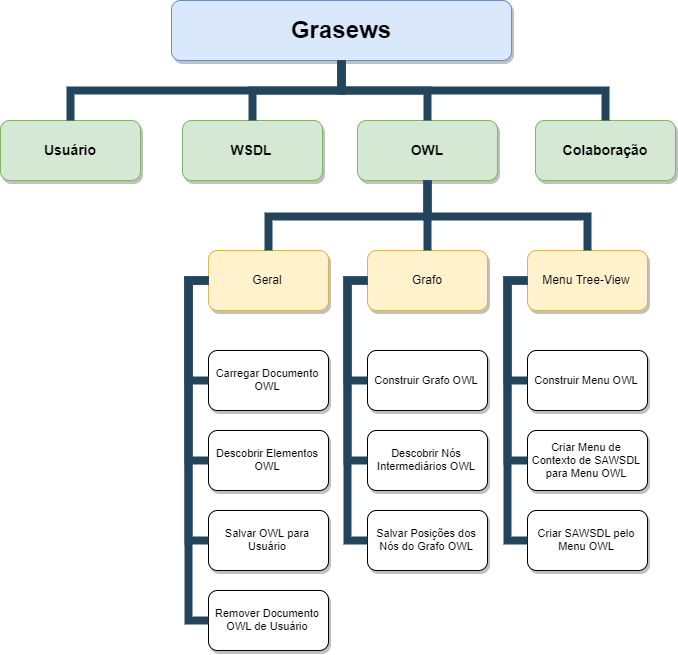
\includegraphics[scale=0.45]{9-pos-textuais/apendices/imagens/grasews-eap-owl.png}
        %}
        \centering
        \caption[Estrutura Analítica de Projetos de Grasews - Parte 3]{\textbf{Estrutura Analítica de Projetos de Grasews - Parte 3.}}
        \label{fig:grasews-eap-owl}
    \end{figure}
%\end{landscape}

%\begin{landscape}
    \begin{figure}[h]
        \resizebox{\textwidth}{!}{
            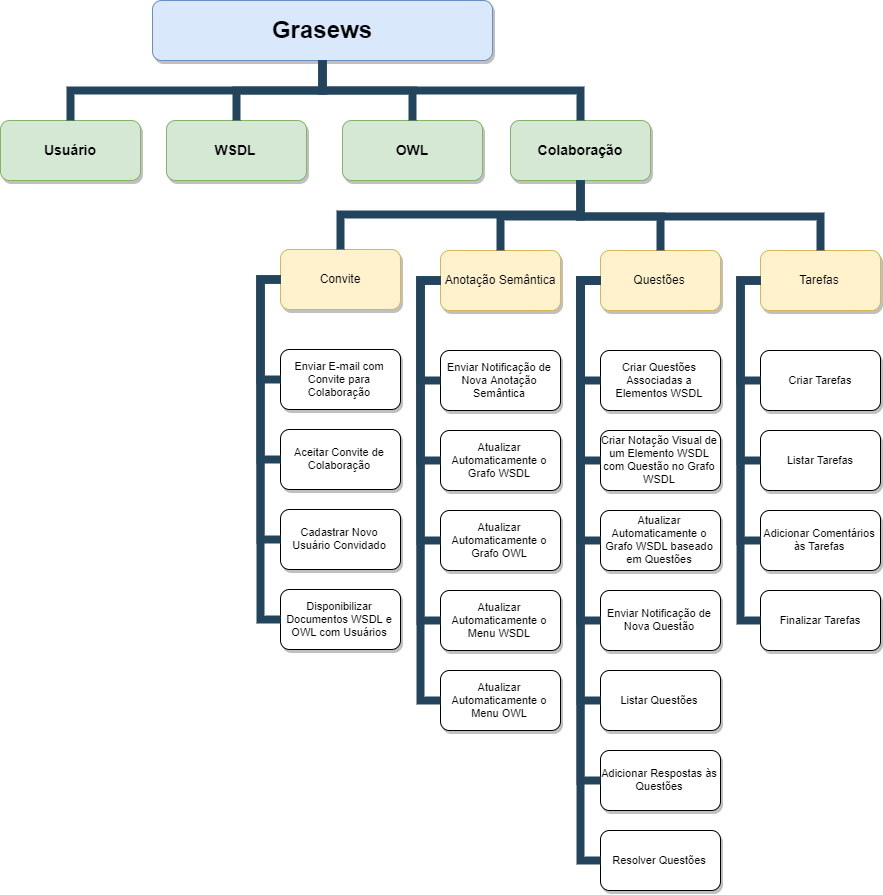
\includegraphics[scale=1]{9-pos-textuais/apendices/imagens/grasews-eap-colaboracao.png}
        }
        \centering
        \caption[Estrutura Analítica de Projetos de Grasews - Parte 4]{\textbf{Estrutura Analítica de Projetos de Grasews - Parte 4.}}
        \label{fig:grasews-eap-colaboracao}
    \end{figure}
%\end{landscape}
%\chapter{Questionário de Avaliação da ferramenta Grasews}\label{apendice-questionario-grasews}

\section{Questionário}

\begin{enumerate}[label=Q\arabic*]

    \item
    \textbf{Quão fácil foi a visualização de descrições de serviços web utilizando o Grasews?}
    \\
    ( ) Muito difícil ( ) Difícil ( ) Indiferente ( ) Fácil ( ) Muito fácil
    
    \item
    \textbf{Quão fácil foi a visualização de conceitos de ontologias utilizando o Grasews?}
    \\
    ( ) Muito difícil ( ) Difícil ( ) Indiferente ( ) Fácil ( ) Muito fácil

    \item
    \textbf{Quão fácil foi a criação de anotações semânticas utilizando o Grasews?}
    \\
    ( ) Muito difícil ( ) Difícil ( ) Indiferente ( ) Fácil ( ) Muito fácil

    \item
    \textbf{Quão fácil foi a visualização de anotações semânticas utilizando o Grasews?}
    \\
    ( ) Muito difícil ( ) Difícil ( ) Indiferente ( ) Fácil ( ) Muito fácil

    \item
    \textbf{Quão fácil foi a realização de um trabalho colaborativo para a criação de serviços web semânticos utilizando o Grasews?}
    \\
    ( ) Muito difícil ( ) Difícil ( ) Indiferente ( ) Fácil ( ) Muito fácil
    
    \item
    \textbf{Se já utilizou outras ferramentas de suporte à anotação semântica, quão mais fácil foi a anotação semântica utilizando o Grasews em relação à(s) outra(s) ferramenta(s)?}
    \\
    ( ) N/A
    \\
    ( ) Muito mais difícil ( ) Mais difícil ( ) Indiferente ( ) Mais fácil ( ) Muito mais fácil
    
    \item
    \textbf{Você acredita que a adoção de serviços web semânticos poderia ser beneficiada se houvesse um suporte ferramental mais adequado?}
    \\
    ( ) Discordo plenamente ( ) Discordo parcialmente ( ) Não discordo e nem concordo
    \\
    ( ) Concordo parcialmente ( ) Concordo plenamente
    
    \item
    \textbf{Você acredita que o Grasews pode contribuir para uma maior adoção de serviços web semânticos?}
    \\
    ( ) Discordo plenamente ( ) Discordo parcialmente ( ) Não discordo e nem concordo
    \\
    ( ) Concordo parcialmente ( ) Concordo plenamente
    
    \item
    \textbf{De 1 (muito ruim) a 5 (muito bom), como você avalia o Grasews?}
    \\
    ( ) 1\hspace{1cm}( ) 2\hspace{1cm}( ) 3\hspace{1cm}( ) 4\hspace{1cm}( ) 5
    
    \item
    \textbf{Tem algum sugestão que possa contribuir com melhorias do Grasews?}
    \\
    ....................................................................................................................................
    \\
    ....................................................................................................................................
    \\
    ....................................................................................................................................
    \\
    ....................................................................................................................................
    \\
    ....................................................................................................................................
    \\
    ....................................................................................................................................
    \\
    ....................................................................................................................................
    \\
    ....................................................................................................................................
    \\
    ....................................................................................................................................
    \\
    ....................................................................................................................................
    \\
    ....................................................................................................................................
    \\
    ....................................................................................................................................
    \\
    ....................................................................................................................................
    \\
    ....................................................................................................................................
    \\
    ....................................................................................................................................
    \\
    ....................................................................................................................................
    \\
    ....................................................................................................................................
    \\
    ....................................................................................................................................
    \\
    ....................................................................................................................................
    \\
    ....................................................................................................................................
    
\end{enumerate}

\section{Resultados}

\section{Conclusão}
\chapter{Tecnologias e Bibliotecas de Desenvolvimento}\label{apendice-tecnologias-grasews}

As principais tecnologias utilizadas no desenvolvimento de Grasews incluem:

\begin{enumerate}

  \item \textbf{Microsoft .NET Framework}
  
  .NET \textit{framework}~\cite{MICROSOFT-2019-NET-FRAMEWORK} é um \textit{framework} de desenvolvimento provido pela \textit{Microsoft}. Todos os módulos e componentes da ferramenta Grasews foram desenvolvidas utilizando a linguagem de programação C\# da versão 4.7 do \textit{framework} .NET. Os tipos de projetos .NET variam entre \textit{Asp.NET MVC}, para o módulo \texttt{Grasews.Web}, \textit{Asp.Net Web API}, para o módulo \texttt{Grasews.API}, e \textit{Class Library}, para os demais módulos da ferramenta.
  
  %Para mais informações, consulte \href{https://dotnet.microsoft.com/download/dotnet-framework/net472}{https://dotnet.microsoft.com/download/dotnet-framework/net472}
  
  \item \textbf{Microsoft ASP.NET MVC}
  
  ASP.NET~\cite{MICROSOFT-2019-ASP-NET-MVC} fornece recursos tecnológicos baseados em padrões para criar \textit{websites} dinâmicos usando o padrão \textit{Model-View-Controller} (MVC). MVC é um padrão de projeto usado para desacoplar a interface do usuário (visualização), os dados (modelo) e a lógica de aplicativo (controlador). Esse padrão ajuda a alcançar a separação de responsabilidades de forma mais clara.
  
  Ao usar o padrão MVC para o desenvolvimento de sites, as solicitações são encaminhadas para um \textit{controller} responsável por trabalhar com um \textit{model} para executar ações e / ou recuperar dados. Um \textit{controller} escolhe a \textit{view} para exibir e fornece o modelo (\textit{model}) para a página. Por fim, uma \textit{view} renderiza a página final com base nos dados de um \textit{model}. O módulo \texttt{Grasews.Web} foi desenvolvido utilizando este recurso.
  
  %Para mais informações, consulte \href{https://dotnet.microsoft.com/apps/aspnet/mvc}{https://dotnet.microsoft.com/apps/aspnet/mvc}
  
  \item \textbf{Microsoft ASP.NET Web API}
  
  \textit{ASP.NET Web API}~\cite{MICROSOFT-2019-WEB-API} é o formato mais recente utilizado para o desenvolvimento de serviços web RESTful do \textit{framework} .NET. O módulo \textit{Grasews.API} foi desenvolvido utilizado este recurso.
  
  %Para mais informações, consulte \href{https://dotnet.microsoft.com/apps/aspnet/apis}{https://dotnet.microsoft.com/apps/aspnet/apis}
  
  \item \textbf{Microsoft .NET Entity Framework}
  
  \textit{Entity Framework}~\cite{MICROSOFT-2019-Entity-Framework} é um \textit{Object Relational Mapper} (ORM) que permite que desenvolvedores trabalhem com um banco de dados por meio de objetos (instâncias de classes). Isso elimina a necessidade da maior parte do código de acesso a dados que os desenvolvedores geralmente precisam escrever, como, por exemplo, sentenças SQL (\textit{queries}). O módulo \texttt{Grasews.Postgres} utiliza \textit{.NET Entity Framework} para o acesso a dados existentes no SGBD \textit{Postgres}.
  
  %Para mais informações, consulte \href{https://docs.microsoft.com/en-us/ef/}{https://docs.microsoft.com/en-us/ef/}
  
  \item \textbf{Simple Injector}
  
  \textit{Simple Injector}~\cite{SIMPLE-INJECTOR-2019} é uma biblioteca de injeção de dependência de código aberto para o \textit{framework} NET. O módulo \texttt{Grasews.IoC} é responsável por controlar as injeções de dependências, suportado pela biblioteca \textit{Simple Injector}.
  
  %Para mais informações, consulte \href{https://simpleinjector.org/}{https://simpleinjector.org/}
  
  \item \textbf{AutoMapper}
  
  \textit{AutoMapper}~\cite{AUTO-MAPPER-2019} é uma biblioteca criada para mapear um objeto para outro. Ao invés de criar um método responsável por mapear propriedades de um objeto para propriedades de outro objeto, uma a uma, \textit{AutoMapper} simplifica o código, deixando o trabalho mais simples para desenvolvedores de \textit{software} utilizando o \textit{framework} .NET. A biblioteca \textit{AutoMapper} é um recurso que provê o padrão de projeto \textit{Adapter}. \textit{AutoMapper} é utilizado na conversão entre objetos \texttt{Models} dos módulos \texttt{Grasews.Web} e \texttt{Grasews.API}, objetos \texttt{DTOs} do módulo \texttt{Grasews.Application} e entidades de domínio do módulo \texttt{Grasews.Domain}.
  
  %Para mais informações, consulte \href{https://automapper.org/}{https://automapper.org/}
  
  \item \textbf{OWIN}
  
  \textit{OWIN}~\cite{OWIN-2019} é uma uma interface padrão de desenvolvimento entre o lado servidor e o lado cliente de uma aplicação desenvolvida com o \textit{framework} .NET. \textit{OWIN} tem o propósito de desacoplar serviços do lado servidor e aplicativos Web desenvolvidos utilizando o \textit{framework} .NET, permitindo uma melhor comunicação entre os módulos \texttt{Grasews.Web} e \texttt{Grasews.API}.
  
  %Para mais informações, consulte \href{http://owin.org/}{http://owin.org/}
  
  \item \textbf{OAuth 2.0}
  
  \textit{OAuth} 2.0~\cite{OAUTH-2019} é o protocolo padrão para autorização de aplicações. \textit{OAuth} 2.0 fornece fluxos de autorização específicos para aplicativos da web, dispositivos móveis e computadores. Os módulos \texttt{Grasews.Web} e \texttt{Grasews.API} utilizam \textit{OAuth} 2.0 para o controle de autenticação e autorização de um usuário de Grasews.
  
  %Para mais informações, consulte \href{https://oauth.net/}{https://oauth.net/}
  
  \newpage
  
  \item \textbf{Microsoft ASP.NET Identity}
  
  \textit{Microsoft ASP.NET Identity}~\cite{MICROSOFT-2019-IDENTITY} é uma biblioteca de desenvolvimento do \textit{framework} .NET que provê suporte a controles de segurança de uma aplicação. Por meio de \textit{Microsoft ASP.NET Identity}, Grasews possui integração com o protocolo \textit{OAuth} e a interface \textit{OWIN}. Os módulos \texttt{Grasews.Web}, \texttt{Grasews.API} e \texttt{Grasews.Security} utilizam a biblioteca \textit{Microsoft ASP.NET Identity}.
  
  %Para mais informações, consulte \href{https://docs.microsoft.com/en-us/aspnet/identity/}{https://docs.microsoft.com/en-us/aspnet/identity/}
  
  \item \textbf{Postgres}
  
  \textit{PostgreSQL}~\cite{POSTGRES-2019} é um sistema banco de dados relacional de objetos de código aberto. O módulo \texttt{Grasews.Infra.Data.EF.Postgres} utiliza bibliotecas de desenvolvimento que proveem conectividade entre \textit{Entity Framework} e \textit{Postgres}.
  
  %Para mais informações, consulte \href{https://www.postgresql.org/}{https://www.postgresql.org/}
  
  \item \textbf{Sentry}
  
  \textit{Sentry}~\cite{SENTRY-2019} fornece uma plataforma de monitoramento de erros baseada na nuvem. \textit{Sentry} possui um conjunto de bibliotecas disponíveis para o \textit{framework} .NET e outras linguagens o qual torna possível capturar erros de uma aplicação e enviar as especificações dos erros para a ferramenta da web. Por meio da ferramenta da web de \textit{Sentry}, o monitoramento e gerenciamento de erros é facilitado. Equipes de desenvolvimento podem mais facilmente descobrir, fazer triagem e priorizar erros em tempo real. Todos os módulos de Grasews utilizam \textit{Sentry} para a captura de exceções.
  
  %Para mais informações, consulte \href{https://sentry.io/}{https://sentry.io/}
  
  \item \textbf{Cytoscape.js}
  
  \textit{Cytoscape.js}~\cite{CYTOSCAPE-2015} é uma biblioteca \textit{JavaScript} para a visualização e análise de grafos. O módulo \texttt{Grasews.Web} utiliza esta biblioteca para a criacão do grafo na interface de usuário. Adicionalmente, o módulo \texttt{Grasews.Cytoscape} é responsável por manipular e construir objetos (modelos), por meio da linguagem de programação C\#, utilizados pela biblioteca \textit{Cytoscape.js}
  
  %Para mais informações, consulte \href{http://js.cytoscape.org/}{http://js.cytoscape.org/}
  
  \item \textbf{Admin LTE}
  
  \textit{Admin LTE}~\cite{ADMIN-LTE-2019} é um modelo de interface de usuário utilizado para a construção de painéis de administração. \textit{Admin LTE} possui o código aberto e disponibiliza diversas variações, customizações e tema de painel de controle. \textit{Admin LTE} fornece uma variedade de componentes responsivos, reutilizáveis e comumente usados em sistemas web. \textit{Admin LTE} é construído sobre o \textit{Bootstrap}. O módulo \texttt{Grasews.Web} utiliza \textit{Admin LTE} em sua interface gráfica de usuário.
  
  %Para mais informações, consulte \href{https://adminlte.io/}{https://adminlte.io/}
  
  \newpage
  
  \item \textbf{Bootstrap}
  
  \textit{Bootstrap}~\cite{BOOTSTRAP-2019} é uma biblioteca de código aberto para o desenvolvimento de aplicações web com HTML, CSS e \textit{JavaScript}. \textit{Bootstrap} fornece um conjunto de componentes responsivos para diversos dispositivos, além de um sistema de grade responsivo, extensos componentes pré-construídos e \textit{plugins} criados no \textit{jQuery}. O módulo \texttt{Grasews.Web} utiliza \textit{Bootstrap}, em conjunto com \textit{Admin LTE} na implementação da interface gráfica de usuário.
  
  %Para mais informações, consulte \href{https://getbootstrap.com/}{https://getbootstrap.com/}

  \item \textbf{jQuery}
  
  \textit{jQuery}~\cite{JQUERY-2019} é uma biblioteca \textit{JavaScript} que simplifica a manipulação de documentos HTML, a manipulação de eventos, animações e o gerenciamento de requisições AJAX. O módulo \texttt{Grasews.Web} utiliza \textit{jQuery} para a construção de funcionalidades da interface gráfica de usuário de Grasews.
  
  %Para mais informações, consulte \href{https://jquery.com/}{https://jquery.com/}
  
  \item \textbf{Font-Awesome}
  
  \textit{Font-Awesome}~\cite{FONT-AWESOME-2019} é uma biblioteca de ícones vetoriais e escaláveis que podem ser personalizados instantaneamente. Tamanho, cor, sombreamento e outras propriedades dos ícones podem ser facilmente modificadas por meio de CSS. O módulo \texttt{Grasews.Web} utiliza ícones providos pela versão 4.7 de \textit{Font-Awesome} para a construção da interface gráfica de usuário de Grasews.
  
  %Para mais informações, consulte \href{https://fontawesome.com/v4.7.0/}{https://fontawesome.com/v4.7.0/}
  
  \item \textbf{CodeMirror}
  
  \textit{CodeMirror}~\cite{CODEMIRROR-2019} é um editor de texto implementado utilizando a linguagem \textit{JavaScript}. \textit{CodeMirror} possui vários modos que dão suporte a manipulação de diversas linguagens de programação. Adicionalmente, \textit{CodeMirror} possui um conjunto de temas CSS que possibilitam customizar o editor de texto. O módulo \texttt{Grasews.Web} utiliza a biblioteca \textit{CodeMirror} no painel de exibição do código WSDL de uma descrição de serviço web na interface gráfica de usuário de Grasews.
  
  %Para mais informações, consulte \href{https://codemirror.net/}{https://codemirror.net/}
  
  \item \textbf{Microsoft SignalR}
  
  \textit{Microsoft SignalR}~\cite{MICROSOFT-2019-SIGNALR} é parte do \textit{framework} .NET que tem como foco a implementação de \textit{web-sockets}. Por meio de \textit{Microsoft SignalR}, aplicações web desenvolvidas em .NET (lado cliente) podem receber atualizações do lado servidor de forma passiva. \textit{Microsoft SignalR} implementa o padrão de projeto \textit{Observer}. Com isso, o lado cliente permanece observando mensagens que são registradas no lado servidor por meio de canais de comunicação denominados \textit{hubs}. Quando uma nova mensagem é registrada em um \textit{hubs}, o lado cliente responde à essa mensagem. \textit{Microsoft SignalR} permite que o módulo \texttt{Grasews.Web} atualize os ambientes de trabalho dos usuários que estão trabalhando de forma colaborativa em uma especificação WSDL aberta na ferramenta. Adicionalmente, além das atualizações dos ambientes de trabalho, os usuários recebem notificações informando-os sobre novas atualizações em uma dada especificação WSDL.
  
  %Para mais informações, consulte \href{https://dotnet.microsoft.com/apps/aspnet/signalr}{https://dotnet.microsoft.com/apps/aspnet/signalr}
  
  \item \textbf{Swagger OpenAPI Specification}
  
  Swagger~\cite{SMARTBEAR-2019-SWAGGER} é uma estrutura de software de código aberto que apoia desenvolvedores a projetar, criar, documentar e consumir serviços da Web RESTful. O módulo \texttt{Grasews.API} provê uma documentação web (\textit{help pages}) com a descrição de suas funcionalidades web por meio do formato \textit{OpenAPI}, automaticamente criado pelo \textit{framework} .NET.
  
  %Para mais informações, consulte \href{https://swagger.io/}{https://swagger.io/}
  
  \item \textbf{JSON}
  
  \textit{JavaScript Object Notation} (JSON)~\cite{JSON-2019} é um formato padrão para troca de dados. JSON é de fácil compreensão tanto para humanos quanto para máquinas. Este formato é completamente independente de linguagens de programação. Toda comunicação realizada entre os módulos \texttt{Grasews.Web} e \texttt{Grasews.API} é realizada por meio de mensagens no formato JSON. Adicionalmente, a construção do grafo por meio da biblioteca \textit{Cytoscape.js} também é feita por meio de objetos no formato JSON.
  
\end{enumerate}



\end{apendicesenv} % descomentar
%\begin{anexosenv}

% Imprime uma página indicando o início dos anexos
\partanexos

\chapter{Artefatos da Prova de Conceito}\label{anexo-artefatos-estudo-de-caso}

\section{Especificação WSDL original}\label{anexo-WSDL-estudo-de-caso}

A \lstlistingname~\ref{lst:estudo-de-caso-wsdl} apresenta o código da especificação WSDL original utilizado pelo estudo de caso no Capítulo \ref{5-estudo-de-caso} deste trabalho. Note que não há anotação semântica alguma e nem a existência do \textit{namespace} de SAWSDL.

\lstinputlisting[language=xml,caption={[Especificação WSDL do estudo de caso]\textbf{Especificação WSDL do estudo de caso}.},label={lst:estudo-de-caso-wsdl}]{9-pos-textuais/anexos/arquivos/movie-original.wsdl}

%\section{Ontologia OWL}\label{anexo-OWL-estudo-de-caso}

%A \lstlistingname~\ref{lst:estudo-de-caso-wsdl-anotado} apresenta o código da especificação WSDL após a anotação semântica realizada pelo estudo de caso no Capítulo \ref{5-estudo-de-caso} deste trabalho.

%\lstinputlisting[language=xml,caption={[Ontologia OWL do estudo de caso]\textbf{Ontologia OWL do estudo de caso}.},label={lst:estudo-de-caso-owl}]{pos-textuais/anexos/arquivos/movieontology.owl}

\section{Especificação WSDL com Anotação Semântica}\label{anexo-WSDL-anotado-estudo-de-caso}

A \lstlistingname~\ref{lst:estudo-de-caso-wsdl-anotado} apresenta o código da especificação WSDL após a anotação semântica realizada pelo estudo de caso no Capítulo \ref{5-estudo-de-caso} deste trabalho.

\lstinputlisting[language=xml,caption={[Especificação WSDL anotada após o estudo de caso]\textbf{Especificação WSDL anotada após o estudo de caso}.},label={lst:estudo-de-caso-wsdl-anotado}]{9-pos-textuais/anexos/arquivos/movie-anotado.wsdl}

\end{anexosenv} % descomentar

%---------------------------------------------------------------------
% INDICE REMISSIVO
%---------------------------------------------------------------------
\phantompart
\printindex
%---------------------------------------------------------------------